
\begin{figure}
\centering
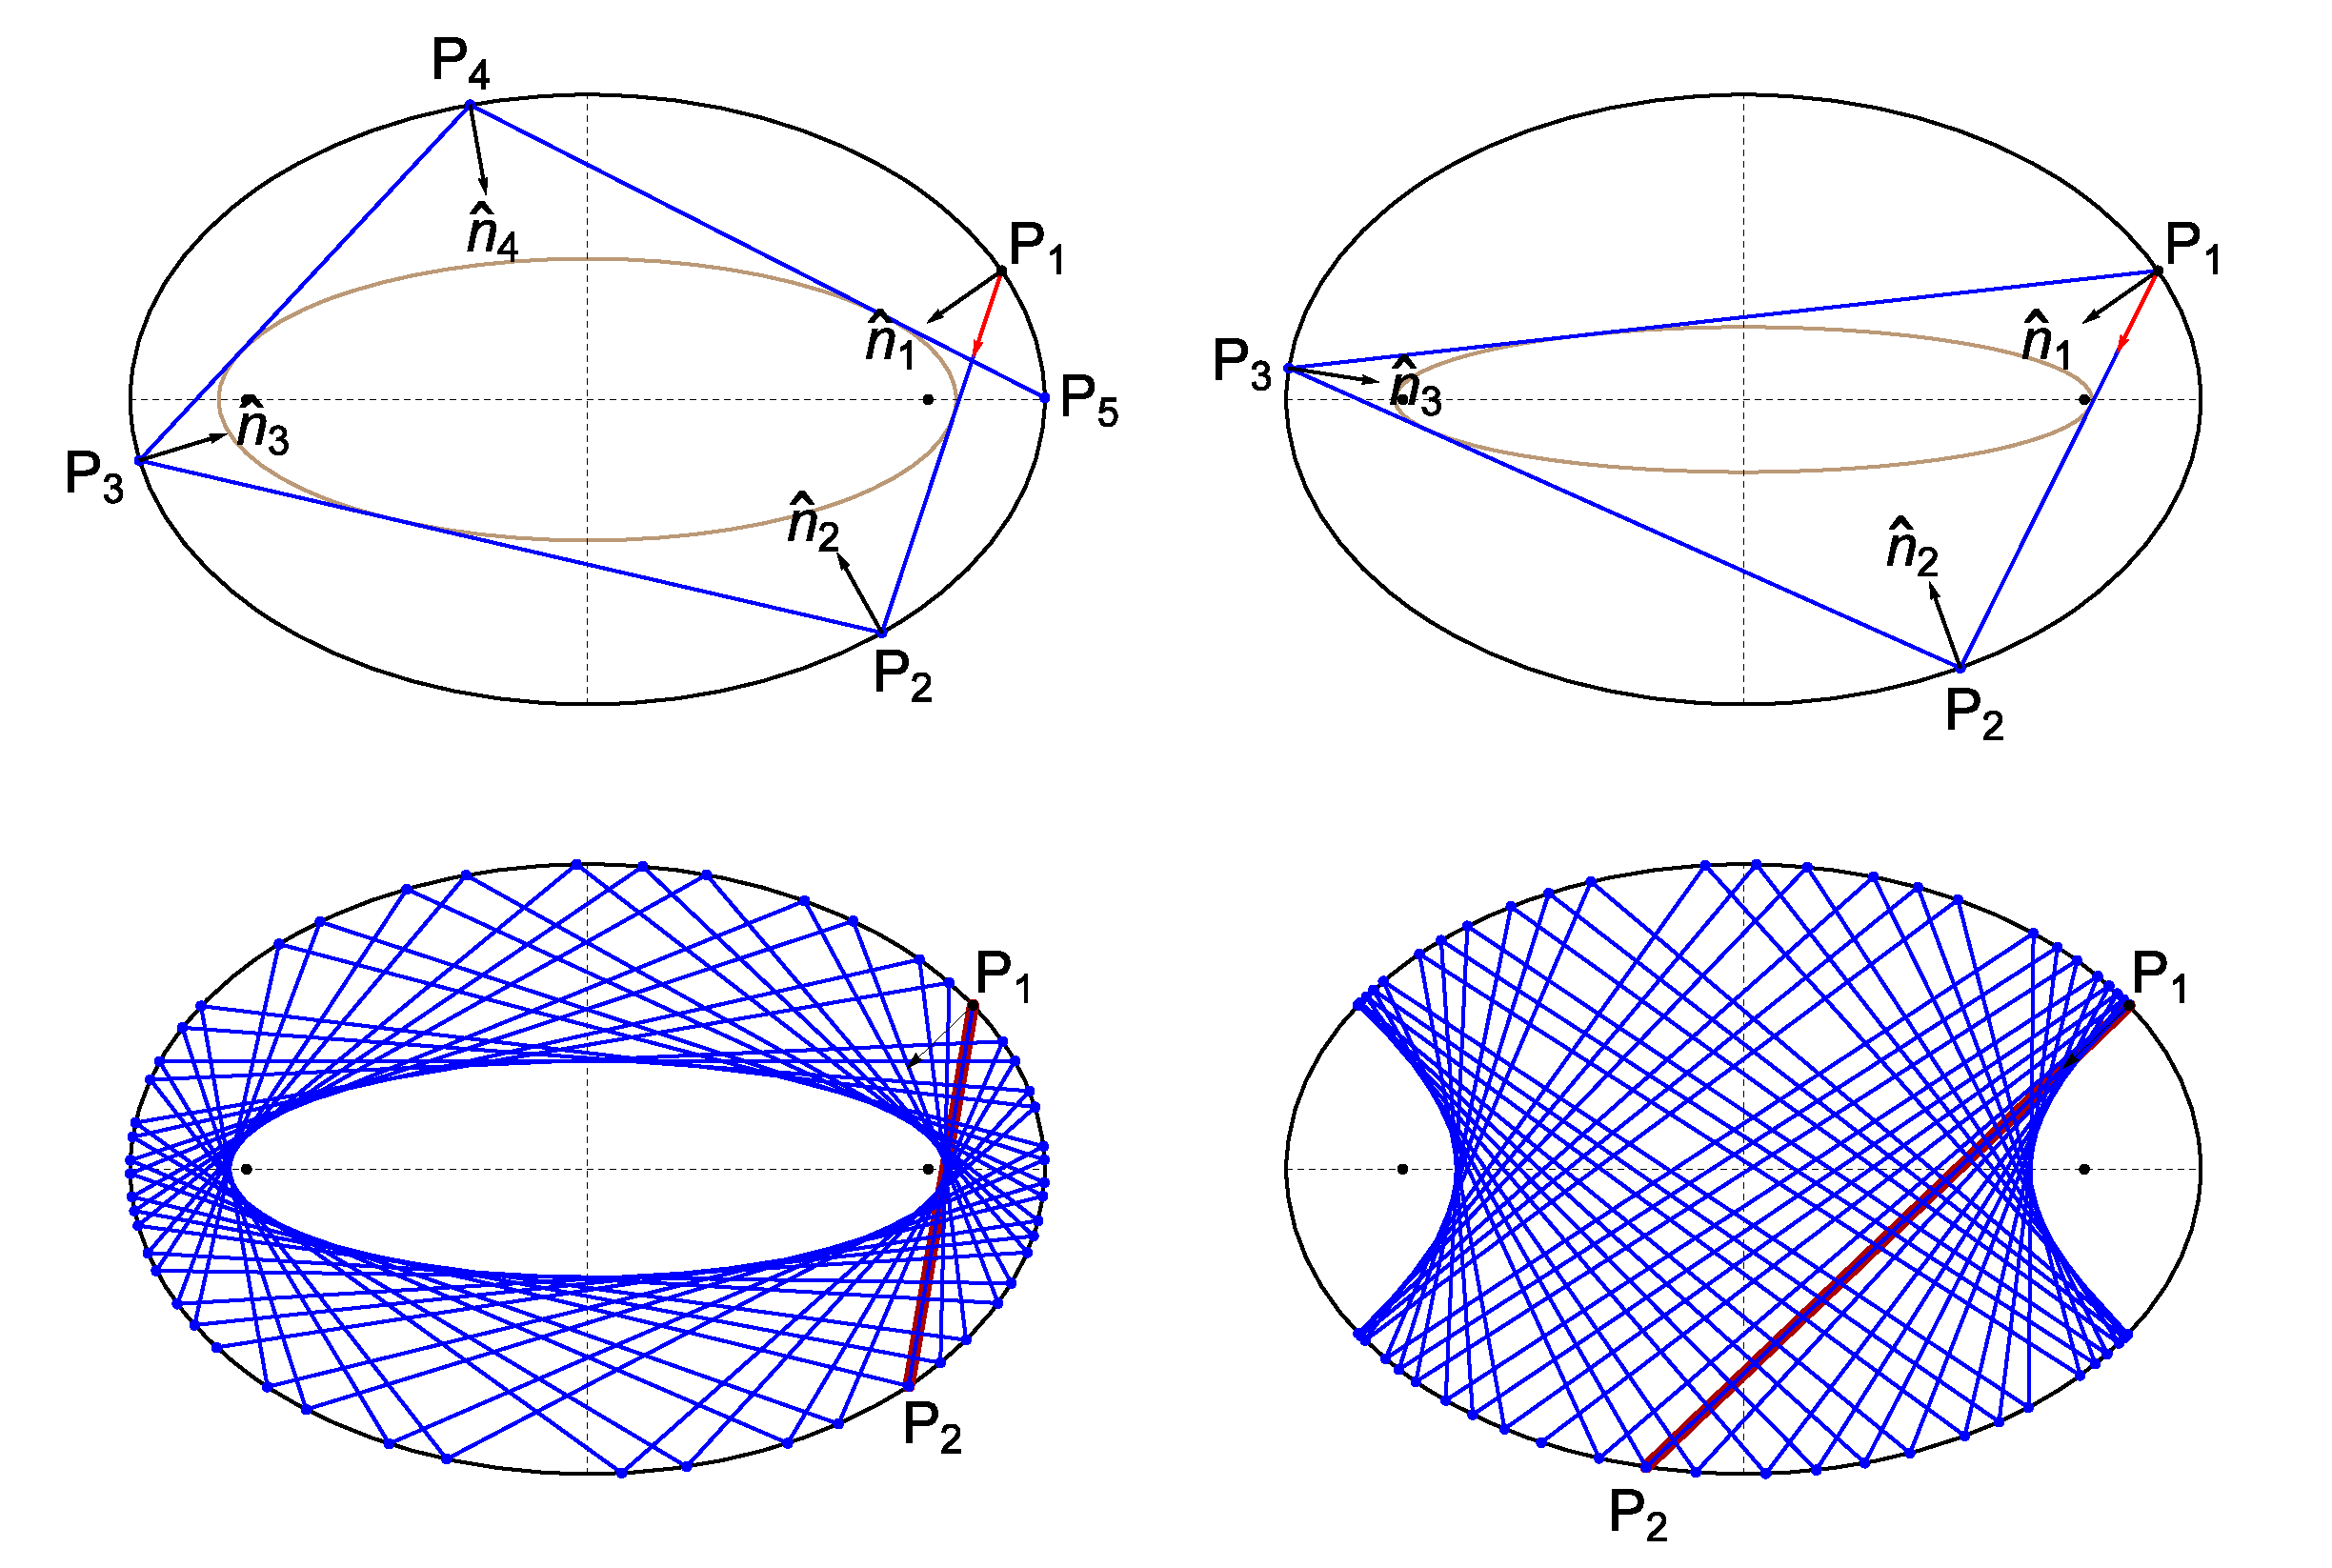
\includegraphics[width=\textwidth]{pics_01_010_billiard_trajectories.eps}
\caption{Trajectory regimes in the elliptic billiard. \textbf{Top left}: The first four segments of a trajectory departing at $P_1$ and moving toward $P_2$, bouncing at $P_i, i=2,3,4$. At each bounce the normal $\hat{n}_i$ bisects incoming and outgoing segments. Joachimsthal's integral \cite{sergei91} means all segments are tangent to a confocal {\em caustic} (brown). \textbf{Top right}: All 3-periodic orbits are tangent to a confocal caustic (brown). \textbf{Bottom}: The first 50 segments of a non-periodic trajectory starting at $P_1$ and directed toward $P_2$. Segments are tangent to a confocal ellipse (left) or hyperbola (right). The former (respectively, latter) occurs if $P_1P_2$ passes outside (respectively, between) the elliptic billiard's foci (black dots). Early \href{https://youtu.be/A7mPzrNJHkA}{Video 1}, \href{https://youtu.be/9zAr5-nm7mw}{Video 2}, \href{https://youtu.be/6yXA0dyWhFY}{Video 3}}
\label{fig:01-billiard-trajectories}
\end{figure}

\begin{figure}
\centering
\begin{subfigure}[t]{0.45\textwidth}
 \centering
 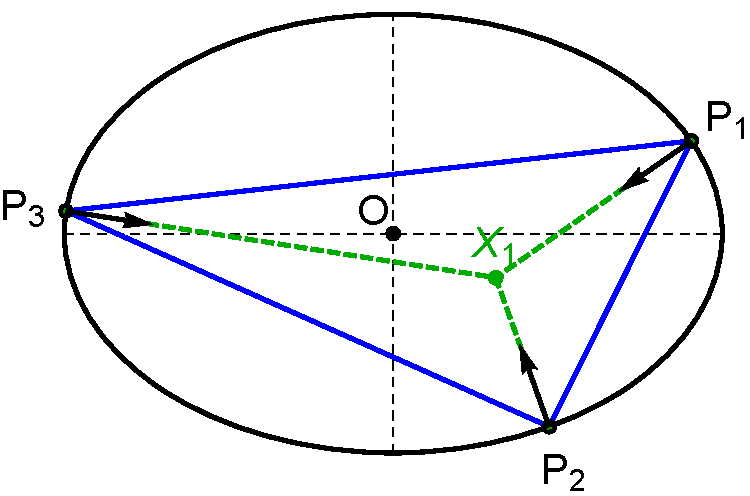
\includegraphics[width=\textwidth]{pics_01_030_single_orbit.pdf}
\end{subfigure}
\hfill
\begin{subfigure}[t]{0.45\textwidth}
 \centering
  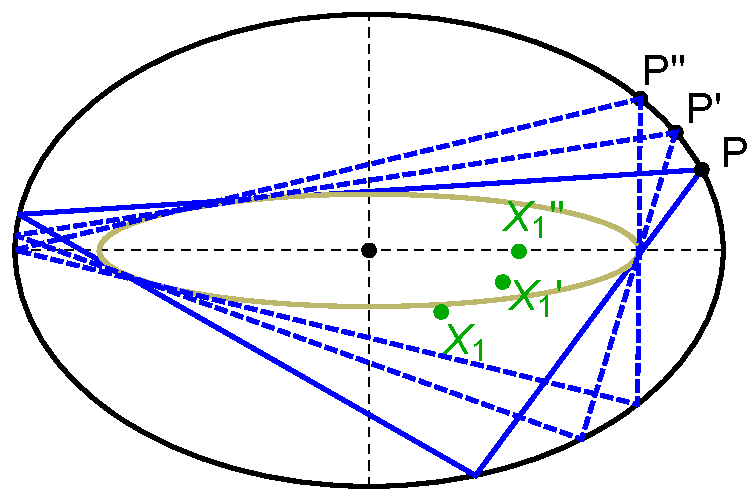
\includegraphics[width=\textwidth]{pics_01_040_three_orbits.pdf}
\end{subfigure}
     \caption{\textbf{Left:} An $N=3$ {\em orbit}. Its incenter $X_1$ is where angular bisectors (black arrows) concur. \textbf{Right}: Three billiard 3-periodics tangent to a confocal caustic (brown). Over positions $P,P',P''$ of a first vertex. Also shown are the corresponding incenters $X_1,X_1',X_1''$.  
\href{https://youtu.be/Y3q35DObfZU}{Video} }
\label{01-basic-n3}
\end{figure}


\begin{figure}
\centering
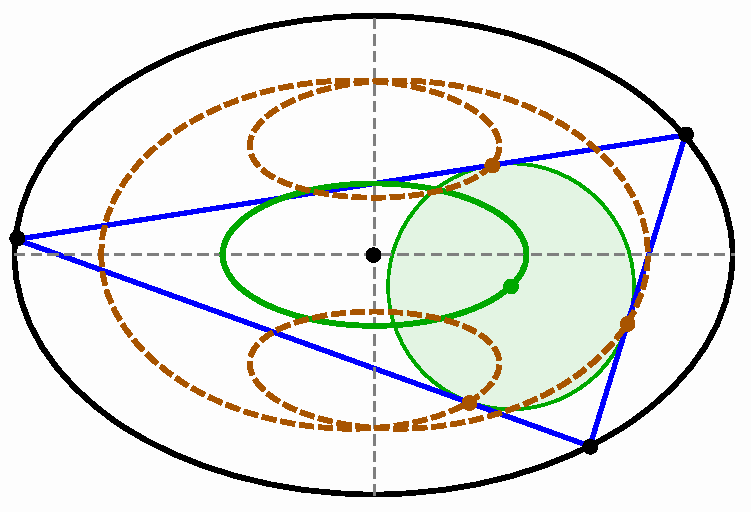
\includegraphics[width=.7\textwidth]{pics_01_020_intouch_locus.pdf}
\caption{An $N=3$ orbit (blue), its Incircle (transparent green), Incenter (green dot) and Intouch Points (brown dots). Over the $N=3$ family, the Incenter locus is a perfect ellipse (green), while the Intouchpoints produce a self-intersecting sextic (dashed brown).
% done
\href{https://youtu.be/9xU6T7hQMzs}{Video}, \href{https://bit.ly/3io8lgN}{Live}}
\label{fig:01-intouch-locus}
\end{figure}

\subsection*{Book Organization}

\begin{itemize}
    \item 
\end{itemize}



